\section{Methods of LSH}
\subsection{Entropy-based LSH}
\cite{panigrahy2006entropy} proposed a method to hash several randomly chosen points in the neighborhood of the query point and showed that at least one of them will hash to the bucket containing its nearest neighbor. The number of randomly chosen points in the neighborhood of the query point $q$ required depends on the entropy of the hash value $h(p)$ of a random point $p$ at distance $r$ from $q$, given $q$ and the locality preserving hash function $h$ chosen randomly from the hash family.

More detailly, let $I(X)$ donate the information-entropy of a discrete random variable $X$. For example, if $X$ takes $N$ possible values with probabilities $w_1, w_2, ..., w_N$, then $I(X)=I(w_1, w_2, ..., w_N)=\sum -w_i\log w_i$. Define $B(p, r)$ as the sphere of radius $r$ centered at $p$. The proposed method tries to retrieve $c$-approximate nerest neighbors of a query point $q$ when giving a distance $r$. Donate $M=I(h(p)|q, h)$, where $p$ is a random point in $B(q, r)$, and $g$ as an upper bound on the probability that two points that are at least distance $cr$ apart will hash to the same bucket, then the algorithm is:
\begin{itemize}
	\item \textbf{Constraction of hash table}: pick $k=\frac{\log n}{\log (1/g)}$ random hash functions $h_1, h_2, ..., h_k$. For each point $p$ in the database compute $H(p)=(h_1(p), h_2(p), ..., h_k(p))$ and store $p$ in a table at location $H(p)$. \textit{polylogn} is used to construct hash tables.
	\item \textbf{Search}: Given $q$ and $r$, pick $O(n^\rho)$ random points $v$ from $B(q, r)$, where $\rho=\frac{M}{\log(1/g)}$, and search in the buckets $H(v)$.
\end{itemize}

The author illustrated that with such an algorithm, the time complexity to find the approximate nearest neighbor is $O(d+n^\rho)$ and the space complexity is near linear.
\subsection{LSH forest}
Since the B+ tree is always accurate, returning exactly the query results, the author tried to combine LSH and B+ tree together to improve accuracy and efficiency on a dynamic set of objects \cite{bawa2005lsh}. The paper aims to design an index structure that enables efficient $\epsilon$-approximate nearest-neighbor queries, the efficient building of the index, efficient insertion and deletion of points, and complete domain independence, all while ensuring minimal use of storage. The proposed methods work for any choice of distance function $D$ for which there is a corresponding LSH family.

The main idea is to encode each data point with variable length hash label $g(p)=(h_1(p), ..., h_k(p))$, where $k$ is different for different $p$ and $k\leq k_m$. Then l prefix trees are constructed on the set of all labels, with each leaf corresponding to a point, and different trees with different hash function sets. In the query procedure, a query for the $m$ nearest neighbors of a point $q$ is answered by traversing the LSH Trees in two phases. In the top-down phase, the leaf $x$ having the largest prefix match with $q$'s label is found by descending each LSH Tree; in the second bottom-up phase, $M$ points from the LSH Forest are collect by moving up from level $x$ towards the root synchronously across all LSH Trees. These two phases are shown in Figure 1. The insertion can be done by simply top-down searching and the deletion top-down and removing the appropriate leaf node.
\begin{figure}
	\begin{center}
		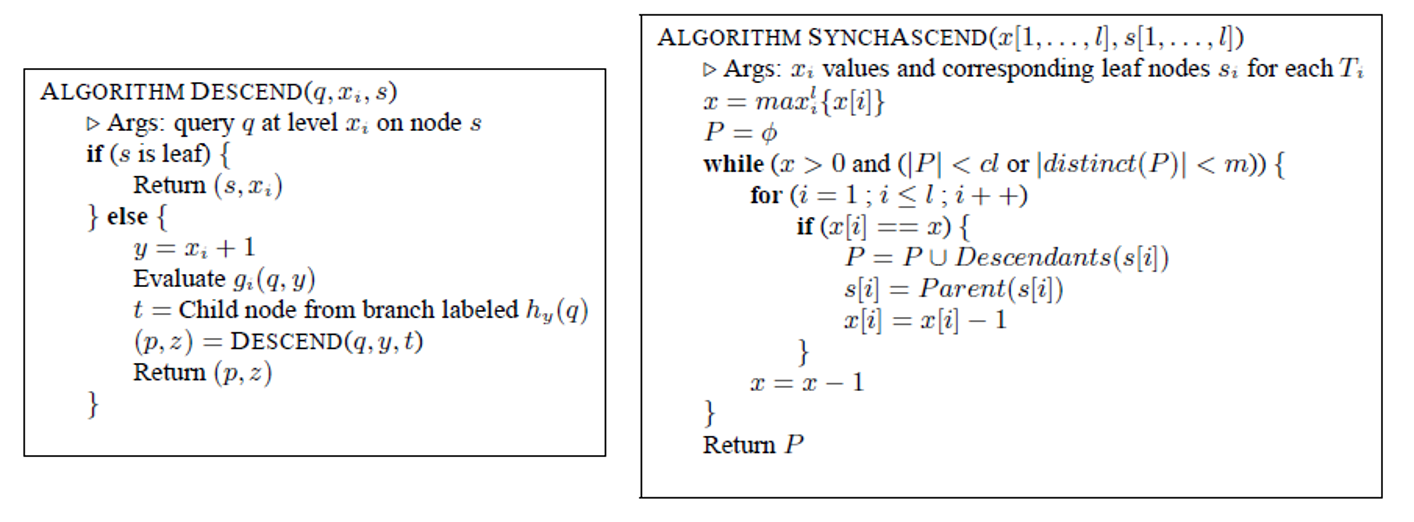
\includegraphics[width=6in]{image/1.png}
		\caption{Top-down and bottom-up phase of LSH Forest query.}
	\end{center}
\end{figure}

The theoretical analysis reveals that the LSH Forest is able to return $\epsilon$-approximate neighbors of a query $q$ with a non-zero probability greater than a constant $C$, as long as the distance from $q$ to its neighbor is in the range $(a,b)$, where the range $(a,b)$ is the definition domain of hash family $H$. 

The author also introduced ways to implement this algorithm in main-memory and disk. In the main-memory implementation, a long chain of logical internal nodes is compressed into just one node that stores the path to it from the previous node to improve storage space. In Disk-based implementation, in order to minimize the number of disk accesses required to navigate down the tree for a query, the Prefix B-Trees is considered as the data structure to construct the LSH forest. The results on peer-to-peer task showing that LSH Forest exhibits higher efficiency than other methods, with higher average similarity and lower mean relative error in a dynamic setting.
\subsection{Adaptative LSH}
This work \cite{jegou2008query} using $E_8$ lattices as hash functions instead of random projections to balance the trade-off between retrieval accuracy and complexity.

A lattice is a discrete subset of $R^d$ defined by a set of vectors of the form $\{x=u_1a_1+...+u_da_d|u_1, ..., u_d\in Z\}$. The $E_8$ lattice can be defined based on another 8-dimensional lattice, the $D_8$ lattice, which is the set of point of $Z^8$ whose sum is even, e.g. $(1,1,1,1,1,1,1,1)\in D_8$. Then $E_8$ lattice is defined as:
$$E_8=D_8\cup (D_8+\frac{1}{2})$$
The author argues that the relevance of the hash function used in LSH is the lower the better. Based on the properties of $E_8$ lattice, the hash functions are defined as $$h_i(x)=E_8(\frac{x_{i,8}-b_i}{w})$$ The detailed algorithm of QA-LSH is exactly the same as the original LSH algorithm, except the hash function family is defined based on $E_8$ lattice, instead of randomly projection. The results indicate that the QA-LSH achieve a higher proportion of nearest neighbors correctly found compared with traditional LSH methods. 

\subsection{Multi-Probe LSH}
Traditional LSH schemes directly return the objects in the exactly collision buckets.
Multi-probe LSH~\cite{lv2007multi} try to probe more buckets in one hash table to reduce the number of hash tables while maintains similar performance.
Formally speaking, multi-probe LSH probes a sequence of buckets which are from the collision bucket and a sequence of perturbations, as \cref{tbl:multi-probe-lsh} shows.
\begin{table}[hbt]
\centering
\caption{Difference between basic LSH and multi-probe LSH}
\begin{tabular}{|c|c|}
\hline
  \textbf{Scheme} & \textbf{Query}\\ \hline
  Basic& $g(q)=(h_1(q), h_2(q), ..., h_M(q))$ \\ \hline
  Multi-Probe& $g(q){+}\Delta^{(i)}, i{=}1,2,...,T$, $\Delta^{(i)}{=}(\delta_1^{(i)}, \delta_2^{(i)}, ..., \delta_M^{(i)})$ \\ \hline
\end{tabular}
\label{tbl:multi-probe-lsh}
\end{table}

Then we are going to introduce how the perturbation sequences are constructed.
\subsubsection{Step-Wise Probing Sequence}
Given the properties of LSH, similar objects are more likely in the close buckets.
This motivates the step-wise probing sequence, which firstly probes all 1-step perturbations, then all 2-step perturbations, and so on.
There are $L{\times} {M\choose n} {\times} 2^{n}$ n-step perturbations in total, where $L$ denotes the number of hash tables and $M$ denotes the number of compound hash functions in each table.

\subsubsection{Query-Based Probing Sequence}
Step-wise probing just consider all coordinates to be equally likely.
However, according the properties LSH, some perturbations are more likely than others.

We consider this hash function: $h(q)=\lfloor\frac{a\cdot q + b}{w}\rfloor$, where $w$ is a fixed hyper-parameter, $a$ is drawn from standard Gaussian, and $b$ is uniformly drawn from $[0, w)$.
For two objects $p, q$, $f(p) - f(q)$ follows Gaussian Distribution, where $f(q){=}a\cdot q {+} b$.
Therefore $P(h(p)=h(q)+\Delta)\approx C \exp(\sum_{i=1}^{M} x_i(\delta_i)^2)$, where $x_i(\delta_i)$ is the distance between q's projection and the boundary, like \cref{fig:x_i} shows.

\begin{figure}[hbt]
\centering
  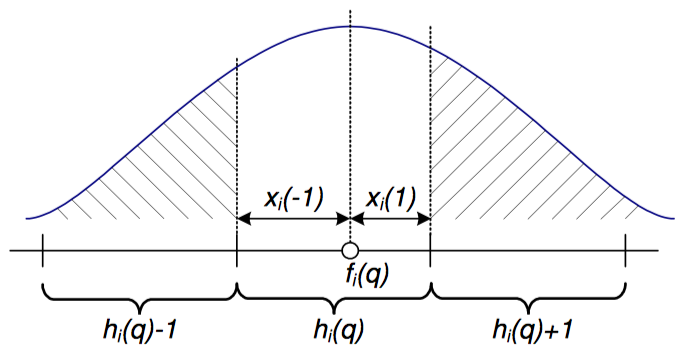
\includegraphics[width=\columnwidth]{figures/multi_probe_nn.png}
  \caption{$x_i(\delta)$}
  \label{fig:x_i}
\end{figure}

In order to find the probing sequence with smallest scores (defined as $score(\Delta)=\sum_{i=1}^{M}x_i(\delta_i)^2$), firstly we need to sort all $2M$ $x_i(\delta_i)$, then we use a heap to generate the probing sequence.

\subsubsection{Optimized Probing Sequence}

One of the drawback of query-based probing sequence is that it needs generating probing sequence for each query.
However, we can use an approximation to precompute it.
We denote the $j$-th elements in sorted $x_i(\delta_i)$ array  as $z_j$, then $z_j$ and $z_j^2$'s expectation is known and independent of query $q$.
Specifically speaking, $E[z_j]{=}\frac{j}{2(M+1)}W, E[z_j^2]{=}\frac{j(j+1)}{4(M+1)(M+2)}W^2$.
We use $\mathbb{E}[z_j^2]$ to replace $z_j^2$, then we only need to sort all $x_i(\delta_i)$ for each query.
\subsection{Dynamic Collision Counting LSH}

Traditional LSH schemes usually use static compound hash function to reduce false positives.
However, the static compound hash functions also reduce recall, and many hash tables have to be used to improve recall.

C2LSH~\cite{gan2012locality} uses dynamic compound hash function rather than a static one.
C2LSH firstly randomly chooses a set of $m$ LSDH functions with appropriately small interval $W$, which form a function base $\mathcal{B}$.
Only data objects with large enough collision counts need to have their distances computed.
A data object is called frequent if its collision number \#collision(o) is greater than or equal to a pre-specified collision threshold $l$.

C2LSH firstly calculate the buckets that $q$ falls in by $h_i(q), i=1,2,...,m$, and find the objects collides with $q$.

Then we compute \#collides(o) for every $o$ and hence identify the set $C$ of all frequent objects. Then we compute $max(\#C, \beta n)$ frequent members of C. $n$ is the the cardinality of the database.
The collision threshold is defined as $l=\alpha m$.
These two properties should hold to ensure C2LSH correct:
\begin{itemize}
	\item $\mathcal{P}_1$: If there exists a data object o, s.t. $o\in B(q, R)$, then o's collision number is at least l. 
	\item $\mathcal{P}_2$: The total number of false positives is less than $\beta n$.
\end{itemize}

In case of no data points returned, it uses virtual reranking to equivalently search a neighbor with radius $1, c, c^2, ...$.
